\documentclass[letterpaper]{article}
\usepackage[utf8]{inputenc}
\usepackage[spanish, mexico]{babel}
\usepackage{amssymb, amsmath}
\usepackage{stackengine}
\usepackage{graphicx}
\usepackage{ mathrsfs }
\usepackage{lipsum}
\usepackage{dsfont}
\usepackage[margin=1.5cm,
vmargin={1.5cm,0.7cm},
includefoot]{geometry}
\usepackage{setspace}
\usepackage{subcaption}
\usepackage{tocloft}
\usepackage{upgreek}
\usepackage{amsthm}
\usepackage{graphicx}
\usepackage{paralist}
\usepackage{fancyhdr}
\usepackage{lmodern}
\usepackage{tcolorbox}
\usepackage{color}
\usepackage{tikz}
\usepackage{wasysym}
\usepackage{textgreek, marvosym}
\tcbuselibrary{skins,breakable}
\pagestyle{fancy}

\renewcommand{\headrulewidth}{0.4pt}
\renewcommand{\footrulewidth}{0.4pt}

\renewcommand{\d}{\partial}

\providecommand{\abs}[1]{\left|#1\right|}
\providecommand{\norm}[1]{\left|\left|#1\right|\right|}														  
\providecommand{\pint}[1]{\langle#1\rangle}														  
\newcommand{\V}{\mathds{V}}

\newcommand{\W}{\mathds{W}}


\newtheorem*{remark}{Recuerde}

\newcommand{\F}{\mathds{F}}

\newcommand{\tq}{ \quad \cdot  \backepsilon \cdot \quad }

\newcommand{\ld}{\lim\limits_{x \to 0^{+}}}

\newcommand{\li}{\lim\limits_{x \to 0^{-}}}

\newcommand{\la}{\lim\limits_{x \to a}}

\renewcommand{\l}{\lambda}

\newcommand{\R}{\mathds{R}}

\newcommand{\Po}{\mathds{P}_2(\mathds{R})}

\renewcommand{\*}{\cdot}

\makeatletter
\renewcommand*\env@matrix[1][\arraystretch]{%
	\edef\arraystretch{#1}%
	\hskip -\arraycolsep
	\let\@ifnextchar\new@ifnextchar
	\array{*\c@MaxMatrixCols c}}
\makeatother

\newtheorem{theorem}{Teorema}[]
\theoremstyle{definition}
\newtheorem{definition}{Definición}


\begin{document}



	\setlength{\unitlength}{1cm}
\thispagestyle{empty}
\begin{picture}(19,3)
\put(-0.5,1.2){
\includegraphics[scale=.20]{img/unam1.png}}
\put(16,1){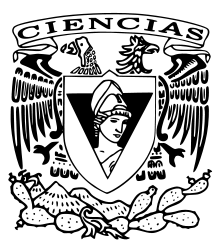
\includegraphics[scale=.29]{img/fciencias1.png}}
\end{picture}

\begin{center}
	\vspace{-114pt}
	\textbf{\large Matemáticas para las Ciencias II}\\
	\textbf{ Semestre 2020-2}\\
	Prof. Pedro Porras Flores\\
	Ayud. Irving Hernández Rosas \\
	\textbf{Tarea Examen III}\\[0.15cm]
	Kevin Ariel Merino Peña\footnote{Número de cuenta 317031326} Armando Abraham Aquino Chapa\footnote{Número de cuenta n}
	José Manuel Pedro Méndez\footnote{Número de cuenta n}\\ [0.12cm]
	\today
\end{center}
\vspace{-10pt}
\rule{19cm}{0.3mm}

\noindent \textbf{Instrucciones:} Realice las siguientes ejercicios escribiéndolos  de manera clara, los puede realizar en \LaTeX, en un cuaderno etc, pero debe de subir el archivo en la sesión de classrroom en formato pdf para su revisión.

%\section*{La integral}

\begin{enumerate}

% -----------------------------------------------------
% Problema uno
% -----------------------------------------------------


\section*{Métodos de integración}

\subsection*{Integración por partes (2.5 pts.)}
\item Realice las siguientes integrales:
\begin{enumerate}
	\item$\displaystyle \int x \sin(x) \, dx$
	\item$\displaystyle \int x^2 e^x \, dx$
	\item$\displaystyle \int x^2 \sin(x) \, dx$
	\item$\displaystyle \int x \ln(x) \, dx$
	\item$\displaystyle \int e^{x} \sin(x) \, dx$
\end{enumerate}

\subsection*{Integración por sustitución (2.5 pts.)}
\item  Realice las siguientes integrales:
\begin{enumerate}
\item$\displaystyle \int \dfrac{\ln(x)}{x} \, dx$
\item$\displaystyle \int e^x \sin(e^x) \, dx$
\item$\displaystyle \int xe^{-x^2} \, dx$
\item$\displaystyle \int x\sqrt{1- x^2} \, dx$
%\item$\displaystyle \int \tan{(x)} \, dx$
\item$\displaystyle \int \dfrac{1}{x \ln(x)} \, dx$
\end{enumerate}

\subsection*{Integración por sustitución trigonométrica (2.5 pts.)}
\item  Realice las siguientes integrales:
\begin{enumerate}
\item$\displaystyle \int \sqrt{1 - x^2} \, dx$
\item$\displaystyle \int \sqrt{x^2 - 1} \, dx$
\item$\displaystyle \int \dfrac{\sqrt{1 - x^2}}{x^2} \, dx$
\item$\displaystyle \int  \dfrac{1}{x^2 \sqrt{1 - x^2}} \, dx$
\item$\displaystyle \int  \dfrac{1}{ \sqrt{x^2 - 1}} \, dx$
%\item$\displaystyle \int x\sqrt{1+ x^2} \, dx$
\end{enumerate}

\subsection*{Integración por fracciones parciales (2.5 pts.)}
\item  Realice las siguientes integrales:
\begin{enumerate}
\item$\displaystyle \int \dfrac{x}{x^2 + 5x + 6} \, dx$
\item$\displaystyle \int \dfrac{x^2 +2}{x(x+2)(x-1)} \, dx$
\item$\displaystyle \int \dfrac{x + 1}{x^2(x-1)^3} \, dx$
\item$\displaystyle \int \dfrac{x^3 - 4x + 3}{x^2(x+1)^2} \, dx$
\item$\displaystyle \int  \dfrac{3x^2 + 1}{(x^2 +1 ) (x^2 + x +1)} \, dx$
%\item$\displaystyle \int \dfrac{3x^2 -1}{(x^2 +1)^2} \, dx$
\end{enumerate}

 \end{enumerate}




\end{document}
